\chapter{Introduction}
\label{ch:introduction}

\section{Motivation}
\label{sec:intro_motivation}
Efficient transportation systems are fundamental to the vitality and accessibility of university campuses, profoundly impacting student life, operational sustainability, and environmental stewardship \cite{dell2016campus, guido2017sustainable}. For an institution such as the Izmir Institute of Technology (IZTECH), which serves a student population of approximately 5500~\cite{iztech_info} spread across the expansive metropolitan area of Izmir, the logistical complexities are considerable. IZTECH, a key technological university, plays a significant role in the educational and research landscape of the region, making the well-being and accessibility for its students a priority. The challenge of designing an optimized transportation network for IZTECH students is multifaceted. It involves not only managing substantial operational costs related to fuel consumption and vehicle maintenance but also enhancing the daily commute for a large, geographically dispersed student body. The inherent difficulties include optimizing routes with fluctuating demand, developing computationally feasible solutions for a large-scale network, and addressing imperfections in real-world data \cite{kaviani2019smart, saberi2017models}. Therefore, optimizing the student transportation network is crucial for improving student experience, ensuring equitable access to education, and promoting the overall efficiency of the university's operations. This thesis endeavors to address these challenges by systematically applying and rigorously evaluating graph theory principles and advanced clustering algorithms to architect an optimized bus routing system tailored for IZTECH students. 
Traditional approaches to transportation network design typically rely on manual determination of routes and schedules. This manual process is time-consuming, often leads to inefficient solutions, and struggles to adapt when student locations change. Transportation planners must make subjective decisions about the number of buses and route assignments, resulting in solutions that may not be optimal or sustainable in the long term.

This thesis presents a parameter-free and adaptive approach that overcomes these limitations. Unlike conventional methods that require extensive manual tuning of parameters such as cluster sizes, route boundaries, and capacity thresholds, our parameter-free approach automatically determines these critical values from the data itself. By using data-driven techniques that automatically configure optimal routes based on student locations, the system can easily adjust to changes without requiring extensive manual replanning or parameter adjustments. This parameter-free nature not only improves efficiency but also ensures better service for all students regardless of where they live. The following chapters demonstrate how this automated, parameter-free approach provides significant advantages over conventional manual planning methods for university transportation systems.

\section{State-of-the-Art}
\label{sec:intro_sota}
The problem of vehicle routing and transportation network optimization has been extensively studied, with a rich body of literature focusing on various methodologies \cite{toth2014vehicle}. Graph theory provides a natural and powerful framework for modeling transportation networks, where locations are represented as vertices and travel segments as edges \cite{tarapata2019graph}.

\subsection{Sparse Graph Representations}
Graph construction techniques are crucial for creating accurate and computationally manageable representations of transportation networks. While complete graphs offer comprehensive connectivity, their $O(N^2)$ complexity is prohibitive for large datasets. Consequently, various sparse graph construction methods have been developed. K-Nearest Neighbors (KNN) graphs \cite{dong2011efficient} connect each vertex to its K closest neighbors, creating a sparse representation that preserves local connectivity. Delaunay Triangulation \cite{lee1980two} creates a triangulation where no vertex lies inside the circumcircle of any triangle, producing a planar graph that captures spatial proximity relationships. Gabriel Graphs \cite{gabriel1969new} connect two points if their diameter sphere contains no other points, resulting in a subgraph of Delaunay that preserves important proximity relationships while being sparser. Other approaches include Relative Neighborhood Graphs \cite{toussaint1980relative}, Minimum Spanning Trees \cite{graham1985euclidean}, and β-Skeletons \cite{kirkpatrick1985framework}.

For our transportation network application, Delaunay Triangulation, Gabriel Graphs, and KNN graphs are particularly advantageous because they strike an optimal balance between sparsity and connectivity. Delaunay preserves natural geographic proximity relationships crucial for transportation routing, while Gabriel offers further sparsification without losing critical connections between nearby student locations. KNN graphs provide flexibility that can be tuned based on the density of student distributions across the metropolitan area.

\subsection{Clustering Algorithms}
Once a graph representation is established, clustering algorithms partition the network into manageable sub-units, which in this context correspond to potential bus routes. Spectral Clustering \cite{ng2001spectral} utilizes the eigenspectrum of graph Laplacian matrices to find optimal cuts, effectively identifying well-separated communities. The Leiden algorithm \cite{leiden}, an improvement over the Louvain method, optimizes modularity to find well-connected communities with enhanced quality and computational efficiency. Multi-view Anchor Graph-based Clustering (MVAGC) \cite{wang2019multi} leverages complementary information from different data representations to achieve more robust clustering. Other notable approaches include K-Means \cite{arthur2007k}, DBSCAN \cite{ester1996density}, Hierarchical Clustering \cite{murtagh2012algorithms}, and Affinity Propagation \cite{frey2007clustering}.

For university transportation networks, Spectral Clustering naturally handles the irregular spatial distribution of student residences across urban environments. The Leiden algorithm offers advantages through its ability to detect communities at multiple scales, important for identifying both dense population centers and more dispersed student groups. MVAGC provides robustness against the inherent noise and variability in real-world geographic data by leveraging multiple perspectives of the network structure.

\subsection{Outlier Detection Methods}
Outlier detection is increasingly recognized as an important pre-processing step in network analysis \cite{lu2020outlier}. K-Nearest Neighbor (KNN) distance-based outlier detection \cite{knn_outlier} identifies outliers based on their distance to their kth nearest neighbor, particularly effective for spatial datasets. Local Outlier Factor (LOF) \cite{breunig2000lof} measures local deviation of density compared to neighbors, detecting outliers in regions of varying density. Additional methods include Isolation Forest \cite{liu2008isolation}, DBSCAN-based detection \cite{ester1996density}, One-Class SVM \cite{scholkopf1999support}, and statistical approaches \cite{barnett1994outliers}.

For our transportation network application, KNN distance-based outlier detection naturally aligns with the spatial nature of the problem—isolated student addresses represent genuine outliers in a geographic context. This method effectively identifies students whose inclusion in regular routes would cause disproportionate detours and increased costs.

\subsection{Shortest Path Algorithms}
Shortest path algorithms determine the optimal travel path within each identified cluster or route. Dijkstra's Algorithm \cite{dijkstra1959note} finds the shortest path between nodes in a graph with non-negative edge weights. A* Algorithm \cite{hart1968formal} extends Dijkstra's by using heuristics to guide the search toward the target. Other approaches include Floyd-Warshall \cite{floyd1962algorithm} for all-pairs shortest paths and Bellman-Ford \cite{bellman1958routing} for graphs with negative edge weights.

This thesis builds upon these state-of-the-art techniques, tailoring and evaluating them for the specific problem of university student transportation. The combination of carefully selected sparse graph representations, clustering algorithms, outlier detection methods, and shortest path calculations addresses the unique challenges of optimizing transportation for a geographically dispersed student population.

\section{Problem Statement}
\label{sec:intro_problems}
Optimizing the student transportation network for IZTECH presents several distinct challenges that this thesis aims to address:

\begin{itemize}
    \item \textbf{Isolated Student Locations:} Assuming that the student addresses localized in specific regions of Izmir,  the addresses that are considerably distant than the majority of the addresses can be called as isolated student locations. These isolated student locations lead to vertices that share fewer edges with other vertices or do not share any edges with the other vertices for a sparse graph construction as it is exemplified in Fig.1.1. These "isolated vertices" complicate route planning, as servicing them can lead to excessively long routes or underutilized buses, thereby increasing per-student transportation costs. Identifying and efficiently integrating or managing these outliers is crucial.
    \begin{figure}[!htbp]
        \centering
        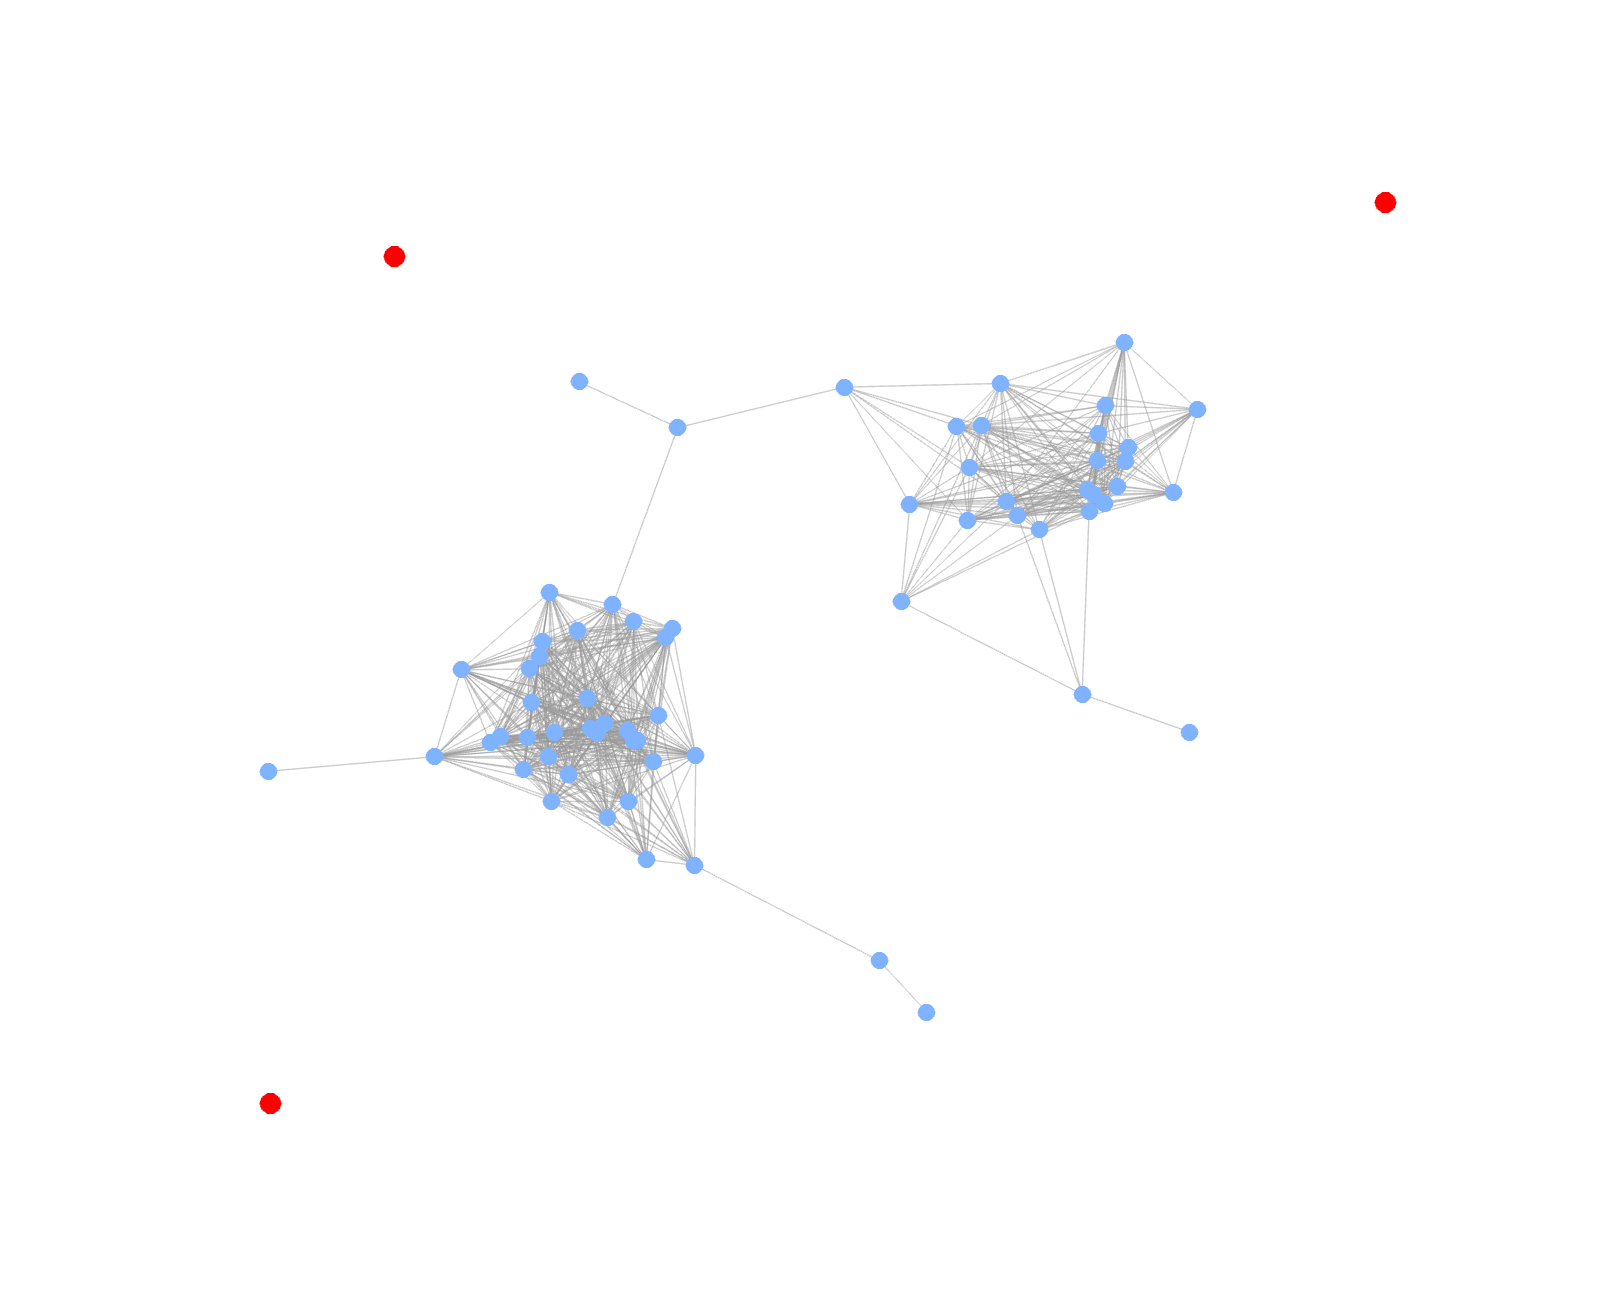
\includegraphics[width=0.9\textwidth]{img/robustness_problem.png}
        \caption{Illustration of the 'Isolated Student Locations' problem. Distant students (highlighted, e.g., in red) can necessitate disproportionately long and costly detours if included in standard routes, impacting overall efficiency.}
        \label{fig:problem_isolated_students}
    \end{figure}

    \item \textbf{Limited Service Capacity:} The university's bus fleet has specific capacity constraints. Each vehicle can typically accommodate a minimum of 10 and a maximum of 50 students. Clustering algorithms and route planning must strictly adhere to these capacity limits to ensure both operational feasibility and cost-effectiveness. Generating routes that are either too small (underutilized) or too large (exceeding capacity) is a key problem.

    \item \textbf{Fuel Consumption and Budget Limitations:} Fuel costs constitute a major portion of the transportation budget. Minimizing total distance traveled by all buses is a primary objective to reduce fuel consumption and operate within budgetary constraints. This necessitates the design of compact and efficient routes.

    \item \textbf{Large Number of Students:} With approximately 2000 students requiring transportation across a large metropolitan area, the scale of the network is substantial, as illustrated in Fig.~\ref{fig:problem_large_scale}. This large number of nodes leads to high computational complexity for many graph algorithms, especially those involving dense matrix operations or exhaustive searches. Scalable and efficient algorithms are therefore essential.
    \begin{figure}[!htbp]
        \centering
        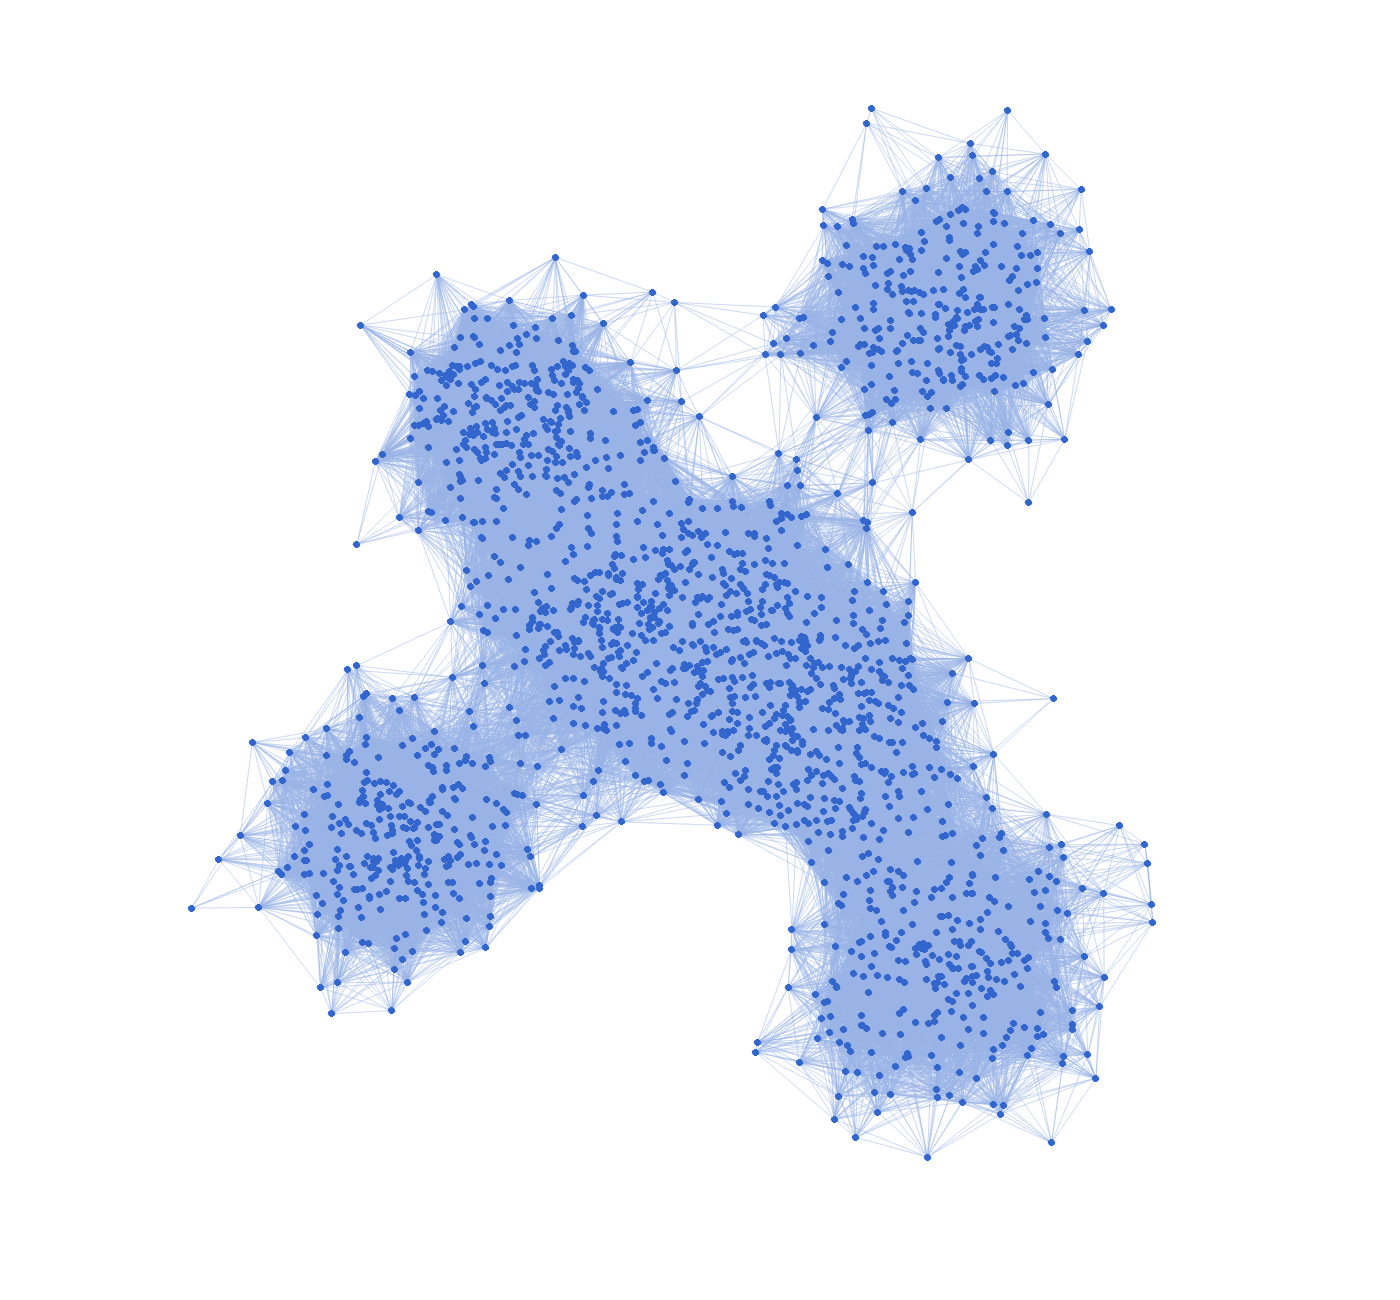
\includegraphics[width=0.7\textwidth]{img/large_scale_students.png}
        \caption{Representing the 'Large Number of Students' problem. The sheer volume and density of approximately 2000 student locations (nodes in the network), as illustrated here, significantly increase the computational complexity of finding optimal routing solutions.}
        \label{fig:problem_large_scale}
    \end{figure}

    \item \textbf{Non-Static Address Information:} While this thesis utilizes a synthetically generated dataset based on current general population distribution, in a real-world scenario, student address information can be non-static, changing every semester. An effective system should ideally be adaptable to such changes, although this aspect is more related to the operationalization than the core algorithmic design focused on here. The current work focuses on optimizing for a given snapshot of student locations.
\end{itemize}
To address all the problems that are listed above, this thesis focuses on an adaptive, robust, computationally efficient and parameter-free service route determination system that is detailed in the sequel.

\section{The Proposed Method}
\label{sec:intro_solution}
This thesis puts forth a solution focused on three primary contributions to optimize the IZTECH student transportation network, each addressing specific challenges outlined in Section~\ref{sec:intro_problems}:

\begin{enumerate}
    \item \textbf{Determining the necessary number of services and alternative solutions:} A key goal is to ascertain the optimal fleet size and explore various route configurations, thereby addressing the issues of Limited Service Capacity by ensuring routes adhere to the 10-50 student limit, and tackling the Large Number of Students by breaking the problem into manageable parts. Our approach achieves this by applying different graph clustering algorithms to partition the student population into potential bus routes, as detailed in Section~\ref{subsec:clustering_sparse}. By comparatively analyzing the outcomes—considering factors like the total number of routes, overall cost (which relates to Fuel Consumption and Budget Limitations), and adherence to capacity constraints—we identify a range of viable solutions and pinpoint the most efficient configurations \cite{zhang2018data}.
    
    \item \textbf{Efficiently determining service routes:} This refers to the development of computationally tractable and cost-effective methods for defining the actual paths for each bus service, directly targeting fuel consumption and budget limitations and the challenge of a large number of students. We begin by employing sparse graph representations (specifically Delaunay Triangulation, Gabriel Graphs, and K-Nearest Neighbors Graphs) of the student network, as described in Section~\ref{subsec:sparse_graph}, which significantly reduces computational complexity. Once students are grouped via clustering, Dijkstra\'s algorithm (Section~\ref{sec:shortest_path}) is utilized to calculate the shortest path connecting students within each group, further minimizing travel distances and defining optimized service routes.
    
    \item \textbf{Ensuring robustness for isolated addresses:} This contribution directly tackles the problem of Isolated Student Locations, where students residing in geographically distant areas could lead to significant inefficiencies. Our solution incorporates a K-Nearest Neighbor (KNN) distance-based outlier detection method as a crucial preprocessing step (Section~\ref{subsec:knn_outlier_application}). This method identifies students whose locations are statistical outliers, allowing them to be handled separately or excluded. This not only improves route compactness, thereby contributing to reducing Fuel Consumption and Budget Limitations, thus enhancing the practicality and cost-effectiveness of the overall transportation plan.
\end{enumerate}

The comprehensive methodology to realize these contributions integrates these specific techniques. It begins with constructing an appropriate graph model of the student network using one of the selected sparse graph methods (Section~\ref{subsec:sparse_graph}). This is followed by the KNN distance-based outlier detection for data refinement (Section~\ref{subsec:knn_outlier_application}). Subsequently, a comparative evaluation of diverse graph clustering algorithms (Spectral Clustering, Leiden Algorithm, and Multi-view Anchor Graph-based Clustering), detailed in Section~\ref{subsec:clustering_sparse}, is performed to partition the students into capacity-constrained routes. Finally, Dijkstra's algorithm (Section~\ref{sec:shortest_path}) determines the optimal path for each route. The interplay between these components—graph construction, outlier detection, and clustering—is analyzed in detail to identify the most effective combination for the IZTECH student transportation problem.

\section{Thesis Overview}
\label{sec:intro_overview}
This thesis is structured to systematically present the research methodology, experimental evaluation, and findings.
\begin{itemize}
    \item \textbf{Chapter~\ref{ch:introduction}} (this chapter) outlines the motivation, discusses the state-of-the-art, defines the problem scope, introduces our proposed solution, and provides this overview of the thesis structure.
    \item \textbf{Chapter~\ref{ch:basics}} provides the necessary theoretical background. It covers fundamental concepts in graph theory, details various graph construction methods and the significance of sparsity, explains the principles behind the selected graph clustering algorithms (Spectral Clustering, Leiden Algorithm, MVAGC), discusses shortest path computation (Dijkstra's algorithm), and introduces the K-Nearest Neighbor distance-based outlier detection technique.
    \item \textbf{Chapter~\ref{ch:method}} details the specific methodologies employed in this research. This includes the generation of the synthetic student dataset, the practical implementation of the different graph construction techniques (Complete, Delaunay, Gabriel, KNN), the adaptation and application of the clustering algorithms to these graphs with capacity constraints, the implementation of the outlier detection process, and the method for shortest path calculation within clusters.
    \item \textbf{Chapter~\ref{ch:experiments}} presents a comprehensive experimental evaluation of the proposed methods. It compares the performance of different combinations of graph construction techniques and clustering algorithms, both with and without outlier detection. The evaluation is based on key metrics including total transportation cost, number of routes, average route length, average cluster size, and computational time. The results are analyzed to identify the most effective and efficient approaches.
    \item \textbf{Chapter~\ref{ch:conclusions}} summarizes the key findings of the research, discusses the main contributions of the thesis to the field of transportation network optimization, and suggests potential avenues for future work, including methodological advancements and practical implementations.
    \item The \textbf{Appendix} may contain supplementary materials, such as detailed experimental results or pseudocode for algorithms not fully detailed in the main text.
\end{itemize}
Through this structured approach, the thesis aims to provide a clear and thorough investigation into optimizing university student transportation networks using graph-based methods.






